\documentclass[11pt]{article}

\usepackage[margin=0.5in]{geometry}
\usepackage{mathtools}
\usepackage{enumerate}

\usepackage{tikz}
\usetikzlibrary{calc,shapes.multipart,chains,arrows}
\usepackage{tikz-qtree}
\tikzset{every tree node/.style={minimum width=2em, minimum height=2em,draw},
         blank/.style={draw=none},
         edge from parent/.style=
         {draw,edge from parent path={(\tikzparentnode) -- (\tikzchildnode)}},
         level distance=1.5cm, sibling distance=0.5cm}


\usepackage{multicol}
\setlength{\columnsep}{0.5cm}
\usepackage{xcolor}

\definecolor{dkgreen}{rgb}{0,0.6,0}
\definecolor{gray}{rgb}{0.5,0.5,0.5}
\definecolor{mauve}{rgb}{0.58,0,0.82}
\definecolor{palegold}{rgb}{0.9, 0.7, 0.6}
\definecolor{darkslategrey}{RGB}{47,79,79}
\definecolor{intellijkeyword}{RGB}{204, 120, 50}
\definecolor{intellijstring}{RGB}{106, 135, 89}
\definecolor{intellijint}{RGB}{104, 151, 187}

\usepackage{hyperref}
\hypersetup{
	colorlinks=true,
	linkcolor=black,
	urlcolor=blue
}

\usepackage{listings}



\lstset{frame=tb,
  language=Java,
  aboveskip=3mm,
  belowskip=3mm,
  showstringspaces=false,
  columns=flexible,
  basicstyle={\small\ttfamily},
  numbers=left,
  numberstyle=\tiny\color{red},
  keywordstyle=\color{intellijkeyword},
  commentstyle=\color{dkgreen},
  stringstyle=\color{intellijstring},
  breaklines=true,
  breakatwhitespace=true,
  tabsize=3,
  otherkeywords={;},
}




\usepackage[parfill]{parskip}

\usepackage{imakeidx}
\makeindex


\begin{document}

\tableofcontents
\newpage

\part{Algoritmer}
\newpage
\section{Hva er en algoritme?}
\subsection{Eksempler}
\subsubsection{Sortere en kortstokk}
Hvordan sortere man en kortstokk er et eksempel på en algoritme.\\
Da trenger man noe å sortere, som da er dataene. \\
Algoritment jobber \textbf{på} dataene. \\

\subsubsection{Filer i en mappe}
Info om filer :
\begin{enumerate}[--]
	\item Filnavn / Filtype
	\item Dato opprettet
	\item Størrelse
	\item Siste Endring
	\item Skrive / lesetilgang
	\item Forfatter
	\item Selve dataene / Innholdet i filen
\end{enumerate}
\paragraph{Algoritmen}

\subsection{Sortere et array}
Speiler koden over.
\begin{enumerate}
	\item Finn største tall
	\item Bytt med første element
	\item Hopp til neste plass, og gjenta
\end{enumerate}

\newpage

\section{Algoritmeanalyse}

Ser på effektiviteten av algoritmer. Utrykkes ofte med "Stor O-notasjon". Dette gir antall operasjoner som må utføres av algoritmen, gitt $n$ antall elementer. \\
\href{https://www.youtube.com/watch?v=dNorFNlDbX0}{Forklaring av O-notasjon : YouTube}

\subsection{Det Harmoniske Tall}
\index{Harmoniske Tallet}Det Harmoniske Tallet ($H_n$) er gitt ved : \\
$H_n = log(n) + 0.577$, der n er antall elementer i imput-arrayet. \\
Dette gir gjennomsnittet av antall tall i arrayet som er mindre enn det minste tallet så langt.

\subsubsection{log(n)}
Gitt \index{logaritme med base 10}logaritme med base 10 :\\
$log(1) = 0 \\
	log(10) = 1 \\
	log(100) = 2 \\
	log(1000) = 3$


\subsubsection{Eksempel}

\begin{lstlisting}
			 
	 	public static int findMax(int[] values) {
			int n = values.length;	 		
	 		
	 		int index = 0;
	 		int max_value = values[index];
	 		
	 		for (int i = 1; i < n; i++) {
	 			if (values[i] > max_value) {
	 				max_value = values[i];
	 				index = i;
	 			}
	 		}
	 		string he = "Hello World";
	 		
	 		return index;
	 	}
	 \end{lstlisting}


Tidsbruken av denne algoritmen vil da skalere med $2n - 1$. Det vil si at det er skalerer lineært med $n$, siden det konstante leddet 1 vil være ubetydelig for store verdier av $n$.


\newpage
\section{Leksikografisk Ordning}

\begin{multicols}{2}
	\raggedcolumns
	Gitt et array [A, B, C, D], vil de neste leksikografiske permutasjonene være : \\
	\begin{enumerate}
		\item[] [A, B, C, D]
		\item[] [A, B, D, C]
		\item[] [A, C, B, D]
		\item[] [A, C, D, B]
		\item[] [A, D, B, C]
		\item[] [A, D, C, B]
	\end{enumerate}
	Dette er da de permutasjoner med A i første-posisjon.

	\columnbreak

	De neste permutasjonene vil da ha B i første-posisjon. \\
	\begin{enumerate}
		\item[] [B, A, C, D]
		\item[] [B, A, D, C]
		\item[] [B, C, A, D]
		\item[] [B, C, D, A]
		\item[] [B, D, C, A]
	\end{enumerate}

\end{multicols}

\subsection{Leksikografisk Sortering som Algoritme}
\href{https://www.youtube.com/watch?v=6FdVfjSmxtA&ab_channel=Andr%C3%A9RiglandBrodtkorb}{Forelesingsvideo}

Hvis vi gir en verdi til hvert element vil vi kunne sette upp grafer for hver permutasjon. \\
...FINN DISSE...

Vi vet at den aller siste permutasjonen (for A-D), vil være [D, C, B, A]. \\
Grafen for dette vil da kun synke. \\
For å ga fra [A, D, C, B] til [B, A, C, D] (altså for å gå til permutasjonen som har et nytt element i første-posisjon).\\
\begin{enumerate}
	\item Søker bakfra langs grafen, til vi kommer til punktet der den ikke lenger er stigende
	\item Finner elementet til høyre for knekk, som er neste større enn A
	\item Bytter om de to elementene (A og B i våre eksempler)

	      [A, D, C, B] $\rightarrow$ [B, D, C, A]
	\item Reverser rekkefølgen på elementer til høre for knekkpunkt

		      [B, D, C, A] $\rightarrow$ [B, A, C, D]
\end{enumerate}

Dette fungerer også for en vilkærlig permutasjon : \\
Gitt [D, A, C, B, E]
\begin{enumerate}
	\item Søker bakfra for å finne knekkpunktet. Her vil E være knekkpunktet.
	\item Finn elementet som er såvidt større enn elementet til venstrre for knekkpunktet. Her er B til venstre, så E vil være elementet som er større.
	\item Bytter om disse to.

		      [D, A, C, B, E] $\rightarrow$ [D, A, C, E, B]
	\item Bytter så neste element med det som er såvidt større til høyre. Dette vil da være C og E.

		      [D, A, C, E, B] $\rightarrow$ [D, A, E, C, B]
	\item Reverserer så elementene til høyre for knekkpunktet.

		      [D, A, E, C, B] $\rightarrow$ [D, A, E, B, C]
	\item Gjentar disse stegene, og får :

	      [D, A, E, B, C] $\rightarrow$ [D, A, E, C, B]
	\item Gjentar nok en gang, og får :

	      [D, A, E, C, B] $\rightarrow$ [D, B, A, C, E]
\end{enumerate}



\newpage
\section{Intervall}
\begin{lstlisting}
		int[] values = {0, 1, 2, 3, 4, 5, 6, 7, 8, 9}

		for (int i = 0; i < 5; i++) {
			System.out.println(values[i])
		}
	
	\end{lstlisting}

\index{Intervall!Halvåpent}
\begin{lstlisting}
		// Jobber i det halvaapne intervallet [begin, end). Altsaa fra og med begin, til (men ikke med) end.
		void func(int begin, int end) {
			for (int i = begin; i < end; i++) {
				pass;
			}
		}
	\end{lstlisting}
\index{Intervall!Lukket}
\begin{lstlisting}
		// Jobber i det lukkede intervallet [left, right]. Altsaa fra og med left til og med right
		void func(int left, int right) {
			for (int i = left; i <= right; i++) {
				pass;
			}
		}	
	\end{lstlisting}
\index{Intervall!Halvåpent}\index{Intervall!Lukket}
\begin{lstlisting}
		// Halvaapent intervall 
		int maks1(int[] a, int begin, int end) {
			pass;
		}
		// Lukket intervall
		int maks2(int[] a, int left, int right) {
			pass;
		}
		
		int[] a = {4, 6, 7, 8, 9, 11, 13, 17}

		int m1 = maks1(a, 2, 6);
		// Jobber paa intervallet fra og med 2 til og med 5. Altsaa [7, 8, 9, 11]

		int m2 = maks2(a, 2, 6);
		// Jobber paa intervallet fra og med 2 til og med 6. Altsaa [7, 8, 9, 1, 13]
	\end{lstlisting}


\newpage
\section{Sorteringsalgoritmer}

\subsection{Bubble-Sort}
En metode som ikke er mye i bruk i dag. \\

Starter bakerst i listen. Ser på to og to elementer. Det elementet som er størst blir plassert forrest av de to.\\

Det vil si at i en liste [1, 4,  2, 7] vil man først se på 2 vs 7, og bytte om på disse to.
Det vil da gi [1, 4, 7, 2].\\ Fra start til slutt får man : \\
\begin{equation}
	\begin{split}
		[1, 4, 2, 7] \\
		[1, 4, 7, 2] \\
		[1, 7, 4, 2] \\
		[7, 1, 4, 2] \\
		[7, 4, 1, 2] \\
		[7, 4, 2, 1]
	\end{split}
\end{equation}

\index{Inversjon}\textbf{Inversjon} : Når to elementer er i feil rekkefølge kalles det en inversjon. \\
Når en liste har 0 inversjoner, er listen sortert.

\begin{lstlisting}
			
			
		\end{lstlisting}

\subsection{Quicksort}
Gitt arrayet [12, 0, 8, 5, 9, 11, 1, 4, 7]. \\

Velger 7 som pivot. Går gjennom listen, og flytter om to og to tall for for å få de på riktig plass i forhold til pivot-tallet. (Her 7)

\textbf{Forelesning}\\
Gitt arrayet [12, 0, 8, 5, 9, 11, 1, 4, 7]. \\
Velger en pivot. Her det siste elementet, 7. \\

Setter venstre og høyre "markører" til start og slutt av arrayet.
Flytter markørene inn mot midten så lenge de oppfyller kravene.\\
I en sortering vil dette være at verdier til venstre er mindre enn pivot,
og verdier til høyre er større eller like pivot. \\
Når dette er gjort vil pivot-verdien ligge på riktig plass i et sortert array. (Den har altså korrekt indeks.) \\

Denne prosessen gjentas til alle verdier er sortert på denne måten. \\

Når man velger pivot er en vanlig strategi å velge den miderste indeksen.
Hvis denne ville blitt et decimaltall, runder man ned.

\begin{enumerate}
	\item Velg et "kort" (verdi) du vil sorterer. (pivot) || O(1)
	      \subitem Ofte miderste verdi.
	\item Plasser alle "kort" som er større enn eller like til høyre.
	      Alle tall som er mindre til venstre. || O(n)
	\item Plasser det valgte "kortet" (pivot) i midten av de sorterte "kortene". || O(1)
	\item Fortsett med del-listene.
\end{enumerate}

\newpage
\section{Søkealgoritmer}

\subsection{Finn Maksverdi}
\begin{lstlisting}
			int[] a = {3, 9, 11, 5, 2, 17, 4};

			int maks(int[] a) {
				int maks_verdi = a[0];

				for (int i = 1; i < a.length; i++) {
					if (maks_verdi < a[i]) {
						maks_verdi = a[i];
					}
				}

				return maks_verdi;
			}
		\end{lstlisting}

\subsection{Finn Minsteverdi}


\subsection{Finn Neste Største Verdi}
\begin{lstlisting}
			int[] a = {3, 9, 11, 5, 2, 17, 4};
			
			int nestMaks(int[] a) {
				int nest_maks = min(a[0], a[1]);
				int maks = max(a[0], a[1]);

				for (int i = 2; i < a.length; i++) {
					if (a[i] > nest_maks) {
						if (a[i] > maks) {
							nest_maks = maks;
							maks = a[i];
						}

						else {
							nest_maks = a[i];
						}
					}
				}
			}
		\end{lstlisting}

\subsection{Søk etter Tall (Usortert)}
Et usortert søk etter et gitt tall.	Returnerer indeksen til tallet det søkes etter.
Hvis tallet ikke eksisterer returneres -1.\\
Dette er en relativt standard måte å søke, siden det ikke finnes noen særlig bedre møter å gjøre dette på.


\begin{lstlisting}
			int[] a = {9, 3, 2, 7, 4};

			int usortertSok(int[] a, int value) {
				for (int i = 0; i < a.length; i++) {
					if (a[i] == value) {
						return i;
					}
				}
				return -1;
			}
		
		\end{lstlisting}

\subsection{Søk etter tall (Sortert)}

Denne funksjonen vil søke fortere med en faktor nesten like steglengden.
Den kan i tilegg bygges rekursivt, det vil si at den / de indre løkkene,
kan utnytte sin egen stenglengde for å ytterlige opptimalisere søket.
\begin{lstlisting}
			int[] a = {2, 3, 4, 7, 9}

			int sortertSok(int[] a, int value) {
				int stepLength = 2;
				for int(i = 0; i < a.length; i = i + stepLength) {
					if (a[i] >= value) {
						int begin = i - stepLength;
						int end = i + 1;'
						for (j = begin; j < n; j++) {
							if (a[j] == value) {
								return j;
							}
						}
					}
				}
				return -1;
			}
		
		\end{lstlisting}

\subsection{Binærsøk}
Deler opp arrayet i 2 deler. \\
Lager Venstre, Høyre og Midtre peker.\\
$v = i_0, h = i_n, m = i_{n/2}$\\

Sjekker om tallet som søkes etter er større eller like midt-tallet. \\
Hvis dette er tilfellet søkes det gjennom det høyre intervallet.
Hvis ikke søkes det i det venstre intervallet. \\

Denne metoden gjentas så for de videre intervall.

\begin{lstlisting}
			int[] a = {2, 3, 4, 7, 9}


		
		\end{lstlisting}

\newpage
\part{Datastrukturer}
\section{Turneringstrær}\index{Datastrukturer!Turneringstrær}
Et turneringstre er en implementering av et binært tre, for å søke gjennom en liste med elementer.
Måten dette gjøres er ved å sette opp et tre som i eksempelet under, og så sammenligne hver node med sin søster-node.
Vinner av denne sammenligningen beveger seg opp til moder-noden. \\

Dette gjør at antall sammenligninger vil bli $n-1$, der n er antall elementer i arrayet.
\subsection{Eksempel}
Turneringstrær brukes for eksempel for å finne maksimum av et tall.\\
\begin{multicols}{2}
	Gitt arrayet [3, 7, 4, 1], får vi treet i første runde. \\\\\\
	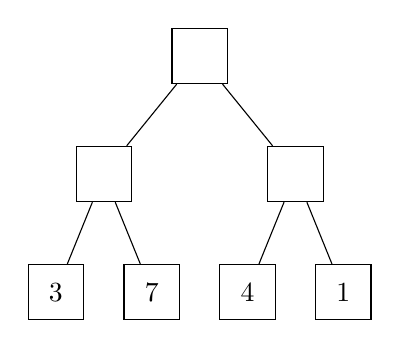
\begin{tikzpicture}
		\Tree
		[.{}
				[.{}
						[.3 ]
						[.7 ]
				]
				[.{}
						[.4 ]
						[.1 ]
				]
		]

	\end{tikzpicture}

	\columnbreak

	Hver kamp blir vunnet av noden med det høyeste tallet, og resultatet blir da : \\\\
	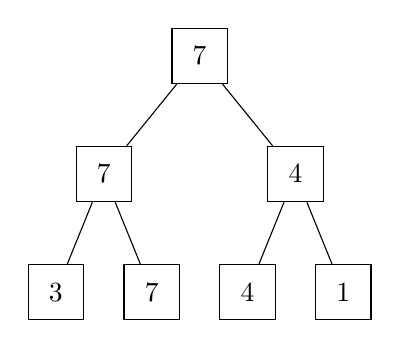
\begin{tikzpicture}
		\Tree
		[.7
				[.7
						[.3 ]
						[.7 ]
				]
				[.4
						[.4 ]
						[.1 ]
				]
		]
	\end{tikzpicture}

	Fra dette kan vi se at 7 er det største tallet i arrayet.
\end{multicols}

\subsection{Turneringstrær i Array}
Gitt treet : \\
\begin{center}
	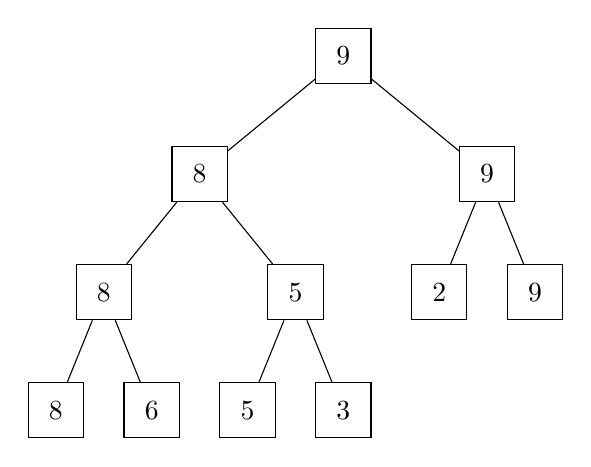
\begin{tikzpicture}
		\Tree
		[.9
				[.8
						[.8
								[.8 ]
								[.6 ]
						]
						[.5
								[.5 ]
								[.3 ]
						]
				]
				[.9
						[.2 ]
						[.9 ]
				]
		]
	\end{tikzpicture}
\end{center}
For å lagre treet i et array gir vi først hver node en unik identifikator (index). Rot-noden starter med en. Hver gang vi går ned til venstre, dobler vi indeksen til moder-noden.
Når vi går til høyre dobler vi indeksen og legger til 1.\\

\newpage
Vi får da : \\
\begin{center}
	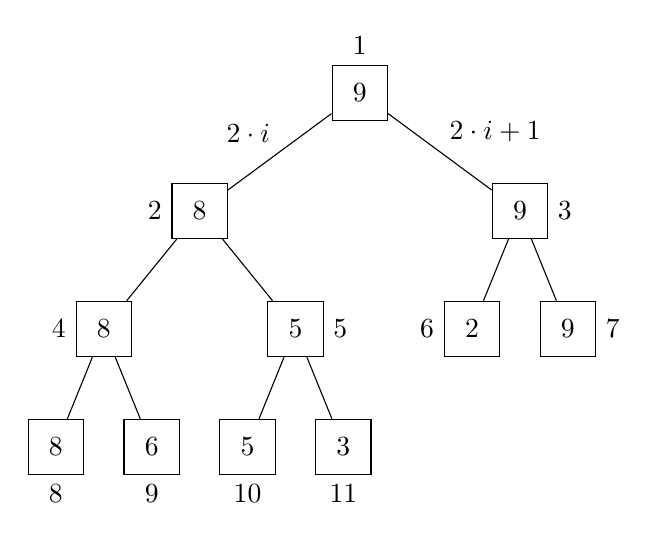
\begin{tikzpicture}
		\Tree
		[.\node [label=above:1] {9};
		\edge node[auto=right] {$2\cdot i$};
		[.\node [label=left:2] {8};
		[.\node [label=left:4] {8};
		[.\node [label=below:8] {8};]
		[.\node [label=below:9] {6};]
		]
		[.\node [label=right:5] {5};
		[.\node [label=below:10] {5};]
		[.\node [label=below:11] {3};]
		]
		]
		\edge node[auto=left] {$2\cdot i + 1$};
		[.\node [label=right:3] {9};
		[.\node [label=left:6] {2};]
		[.\node [label=right:7] {9};]
		]
		]
	\end{tikzpicture}
\end{center}

Vi bruker så disse indeksene til å plassere treet i et array, og får da :
$[Null, 9, 8, 9, 8, 5, 2, 9, 8, 6, 5, 3]$

Fremgangsmåten for å komme frem til dette er ved å først plassere start-verdiene på sine respektive plasser i arrayet.\\
Da får man int[] = $[Null, Null, Null, Null, Null, 5, 2, 9, 8, 6, 5, 3]$ \\
Deretter går man bortover indeksene, og bruker formelene inversene av  $2\cdot i$ og $2 \cdot i + 1$ for å finne hvilke noder som konkurrerer om plassen.\\
Her har den første åpne plassen index = 5. Da får vi $5 \cdot 2 = 10$ og $5 \cdot 2 + 1 = 11$. \\
Det er altså nodene med index 10 og 11 som konkurrerer. \\
Fra det ser vi at node 10 vinner, da dene inneholder den største verdien. \\
Arrayet blir da $[Null, Null, Null, Null, Null, 5, 2, 9, 8, 6, 5, 3]$ \\
Dette kan så gjentas for hver posisjon i arrayet til hele turneringen er ferdigspilt. \\

Dette vil også si at vi aldri bruker det faktiske treet i koden, siden input vil være et array. \\

\subsubsection{Eksempelkode}

\begin{lstlisting}
				
				int[] a = [Null, Null, Null, Null, Null, 5, 2, 9, 8, 6, 5, 3]

				for (int i = begin; i > 0; i++) {
					int id = i;
					int left = 2 * id;
					int right = 2 * id + 1;

					if (a[left] > a[right]) {
						a[id] = a[left];
					}

					else {
						a[id] = a[right];
					}
				}

			\end{lstlisting}
\subsection{Turneringstrær som Noder}

Et turneringstre kan også lagres som en samling med noder.
Der vil nodene refere videre til sine child-noder. Det vil si at alle noder
referer til 0, 1 eller 2 noder.

\subsubsection{Eksempelkode}
\begin{lstlisting}
				public class Node {
					char value;
					Node left_child;
					Node right_child;

					
				}	
			
			\end{lstlisting}

\newpage
\section{Linked List}
En lineær datastruktur. Dette vil si at dataen ikke er lagret i sammenhengende
plasseringer i minne. Dette betyr at hvert element i strukturen må kjenne til plasseringen til det neste elementet.
(Potensielt også det forrige elementet.) \\

Elementene kalles som regel \textit{noder}. En node vil på det minste inneholde en variabel
med data, og en variabel med palsseringen til den neste noden. \\ \\
\subsection{Eksempel på struktur}
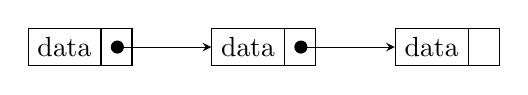
\begin{tikzpicture}[list/.style={rectangle split, rectangle split parts=2,
				draw, rectangle split horizontal}, >=stealth, start chain]

	\node[list,on chain] (A) {data};
	\node[list,on chain] (B) {data};
	\node[list,on chain] (C) {data};
	\draw[*->] let \p1 = (A.two), \p2 = (A.center) in (\x1,\y2) -- (B);
	\draw[*->] let \p1 = (B.two), \p2 = (B.center) in (\x1,\y2) -- (C);
\end{tikzpicture}


\newpage

\section{Definisjoner}

\index{Leksikografisk Sortering}\textbf{Leksikografisk Sortering} : Å sortere data som om de står i et leksikon.\\
For arrays med tall 1 til 5 vil [1, 2, 3, 4, 5] det minste / første, og [5, 4, 3, 2, 1] det største / siste elementet.

\index{Permutasjonsnummer}\textbf{Permutasjonsnummer} : I leksikografisk sortering er dette nummeret for en gitt permutasjon, basert på hvilket nummer det er i listen over alle mulige permutasjoner.\\
For eksempel vil [1, 2, 3] ha permutasjonsnummer 1, [1, 3, 2] er 2, og [2, 1, 3] 3.

\index{Intervall!Halvåpent}\textbf{Halvåpent Intervall} : Skrives som [begin, end). Er intervallet fra og med begin, til men ikke med end.

\index{Intervall!Lukket}\textbf{Lukket Intervall} : Skrives som [left, right]. Er intervallet fra og med left, til og med right

\index{Harmoniske Tallet}\textbf{Det Harmoniske Tallet} : Er gitt ved $H_n = 1 + \frac{1}{2} + \frac{1}{3} + \dots + \frac{1}{n}$ og approksimeres med $H_n\approx log(n) + 0.577$, der n er antall elementer i et array.
Det Harmoniske Tallet sier hvor mange elementer i et array som i snitt vil være mindre enn det minste elementet så langt.

\printindex
\end{document}